%!TEX root = ../../report.tex

\subsection{Shape Grammars} % (fold)
\label{ssub:shape_grammars}


Shape Grammars can be considered grammars for design. In stead of having symbols or letters as components of the alphabet, it has shapes that can be in 2D or 3D. And have production rules that are composed by this shapes, that specify the evolution of the system. With this process, similar to the L-Systems explained before, the shape starts from a seed, i.e. a usually simple shape and can evolve to one big and/or complex shape.

The process is performed in two steps, the recognition of a shape and the replacement according to the rules that are previously defined. 

The Figure~\ref{fig:SGrammars} exemplify one shape grammar, with one rule and the evolution of the application of this rule to the shapes iteratively. In this image, it's shown that from very simple initial shape, can be generated a complex from with a few iterations.

\begin{figure}
        \centering
		\begin{subfigure}[b]{0.55\textwidth}
			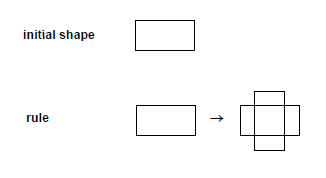
\includegraphics[width=\textwidth]{img/Theory/Shape_Grammars/Grammar.png}
			\caption{a)}
			\label{fig:SGGrammar}
		\end{subfigure}
        
         %add desired spacing between images, e. g. ~, \quad, \qquad, \hfill etc.
          %(or a blank line to force the subfigure onto a new line)
		\begin{subfigure}[b]{0.55\textwidth}
			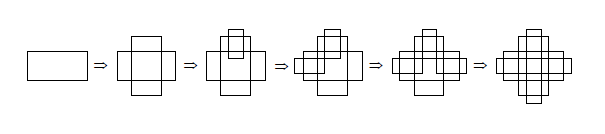
\includegraphics[width=\textwidth]{img/Theory/Shape_Grammars/Recursion.png}
			\caption{b)}
			\label{fig:SGRecursion}
		\end{subfigure}
        \caption{a) Grammar Tiles b) Recursion steps}
        \label{fig:SGrammars}
\end{figure}

This is applied to the generation of buildings in the CityEngine \ref{sub:cityengine} system, using 3D blocks for the main form, and 2D shapes to design the facades.

% \begin{figure}[htbp]
% 	\centering
% 	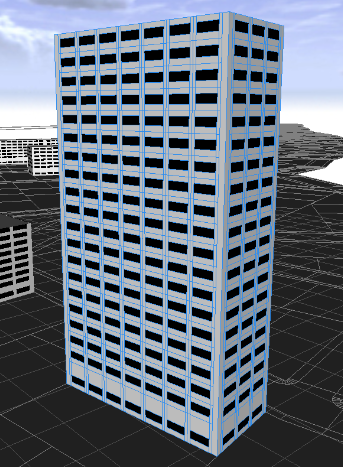
\includegraphics[width=0.55\textwidth]{img/Theory/Shape_Grammars/Edificio.png}
% 	\caption{Simple Building}
% 	\label{fig:SGBuilding}
% \end{figure}

The Figure~\ref{fig:SGBuilding} shows a simple building that I modelled using CityEngine and it's CGA Shape Grammar. But CGA is powerful enough to model much more complex buildings like the Figure~\ref{fig:CEBuilding}.


% \begin{figure}[htbp]
% 	\centering
% 	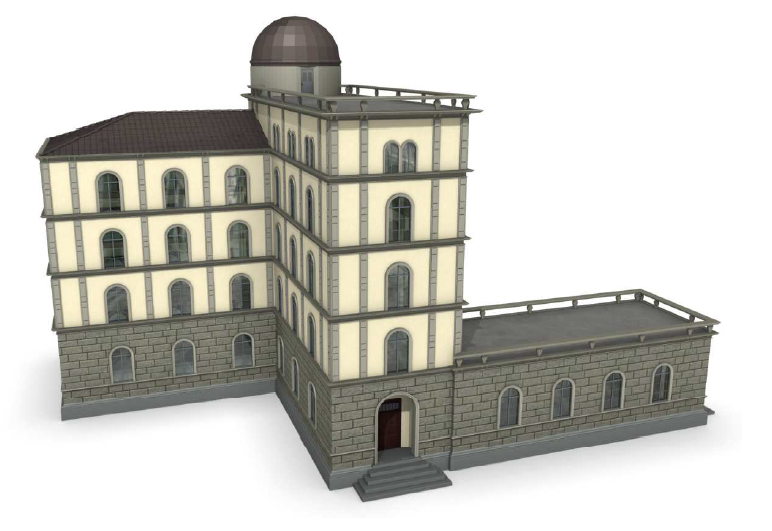
\includegraphics[width=0.55\textwidth]{img/Theory/Shape_Grammars/Capturar.png}
% 	\caption{Complex Building \cite{Muller2006}}
% 	\label{fig:CEBuilding}
% \end{figure}

\begin{figure}
\centering
\begin{minipage}{.5\textwidth}
  \centering
  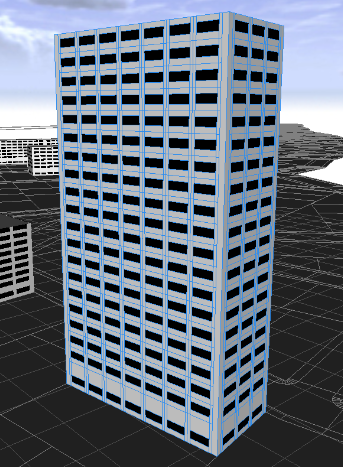
\includegraphics[width=.5\linewidth]{img/Theory/Shape_Grammars/Edificio.png}
  \captionof{figure}{Simple Building}
  \label{fig:SGBuilding}
\end{minipage}%
\begin{minipage}{.5\textwidth}
  \centering
  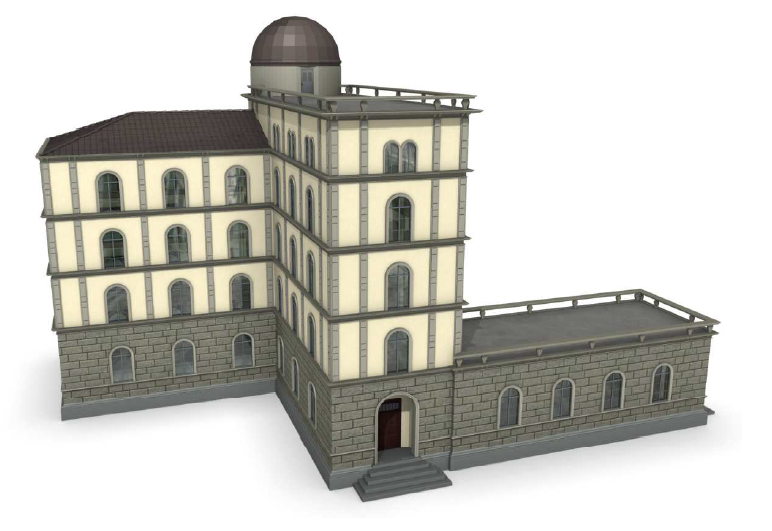
\includegraphics[width=.8\linewidth]{img/Theory/Shape_Grammars/Capturar.png}
  \captionof{figure}{Complex Building \cite{Muller2006}}
  \label{fig:CEBuilding}
\end{minipage}
\end{figure}

% subsubsection shape_grammars (end)